% Chapter Template

\chapter{Summary and personal Evaluation} % Main chapter title

\label{Chapter9} % Change X to a consecutive number; for referencing this chapter elsewhere, use \ref{ChapterX}
\section{Project management}
The project management is divided into four parts based on the timeline: before Christmas vacation, during Christmas vacation, before Easter vacation, and during Easter vacation (Because deadline has been extended to April 24th, more testing will be done during that period).
\\
The Gannt Chart for Hybrid Desktop is shown like the following figure:
\begin{figure}[h]
    \centering
	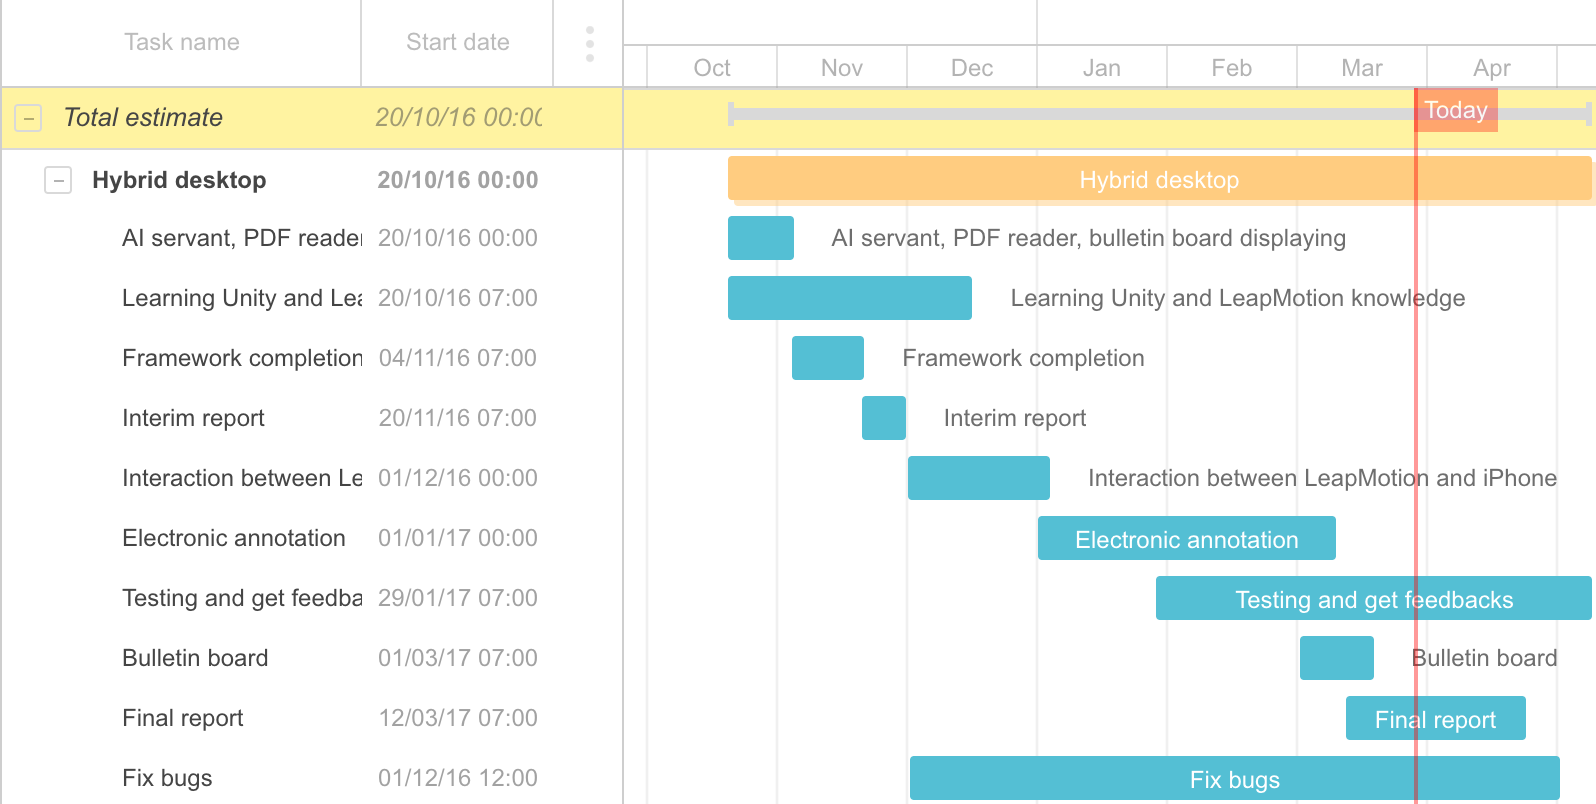
\includegraphics[width=\textwidth]{gann}
    \caption{Gannt Chart for Hybrid Desktop project management}
    \label{fig:mesh1}
\end{figure}
\\
Before Christmas vacation, the main goal is to define the requirements and design the structure and framework of the project. Meanwhile, it is also very significant to learn Unity techniques and Leap Motion API. Some basic implementation like AI servant, PDF reader and bulletin board displaying should be done. Complete the framework of the project, obtain the necessary knowledge of Unity and Leap Motion and finish the interim report before the Christmas vacation. 
\\
\\
During the Christmas vacation, time is much more sufficient, so some challenging goals, such as, exploring the interaction between Leap Motion and iPhone can be appointed, and using this new technique to perform interaction with the PDF reader. Another challenging goal is electronic annotation, during the Christmas vacation, trying to do some literature surveys and reading some articles related with this idea to explore a better solution for this problem.
\\
\\
Before the Easter vacation, because some functionalities have been implemented, the main goal is to do some tests with students, get feedbacks from them, list some improvements and modify the program. During this period, there are weekly lectures, the time is relatively tight. So, another task is completing the bulletin board which is necessary but not so challenging. Meanwhile, implementing the AI servant and adjust its functionality based on user feedback, such as what other information that students hope they can get from the AI servant. At this stage, the project should be almost completed. Final report should be started to write. Complete each chapter, get feedback from the supervisor, and improve it each week.
\\
\\
During the Easter vacation, the main goal should be get feedback from students continuously, fixing bugs and perfect the final report. There should be no major change to the project, and the most important thing is to ensure this project works well and will not cause any crash.

\section{Self reflection}
Personally, I feel this hybrid desktop project is a success, as it solved the main issue which is conceived to solve. And it meets all the functional and non-functional requirements which are listed at the start of the project, and the feedbacks which I get from the prospected users (university students) are almost positive. Another reason that I believe this project was successful is that I explored the Leap Motion by myself, implemented some new features to meet the new requirement and I really feel enjoyable through this experience.
\\
\\
During this project, I learned a lot from my supervisor. At the start of the project, I was totally interested in the Mixed reality but had no experience in this aspect. My supervisor and I have weekly meetings, I expressed my ideas and talked about the hybrid desktop in my mind and some prospected functionality it should have. Supervisor gives me feedback and email some useful websites and articles to me. I growed very quickly through this experience. And it laid the foundation for my further implementation. Talking more with supervisor and do some demos are two important lesson which I learn from this project. It is not only a way to show what you are doing, but also a direct way to learn what can I improve and how can I improve.
\\
\\
It is the largest project that I had ever worked all by myself. From design to implementation, I use some clever method like Gantt chart to divide my time and make periodic goal. Every week, I have specific tasks to do, and this well-arranged plan makes the project go well.
\\
\\
One of the areas I feel was weak in this project, was the research part. I think my literature survey about the Leap Motion and Unity is not enough. Leap Motion and Vuforia are still new for most developers, so there are limited sources about it on the Internet. When I face some difficulties, it always costs a long time to search for an answer and trying to figure it out. And I should do deeper comparison for the choice of programming language as well, during my development, I changed my language because some problems arise later. And this should not happen, I need to plan it well at the beginning of the project.
\\
\\
If I could work on this project again, there are several changes that I will make. Firstly, I need to define a more rigorous framework and design of the project. So, I will not face some problem which may caused by the unsuitable choice of the programming language. Secondly, I will think about the user test through my development. Because in this project, I started to consider the what should I test with the students when I almost finished most functionalities, and it may let me miss something. It should be much better if I consider it earlier. Next time, during my development, after I finish each task, I will store it and when I need to do user test, I can check these functionalities easily and help me to design more structured user tests.
